\documentclass[12pt]{article}

\usepackage{url}
\usepackage{amsmath}
\usepackage{float}
\usepackage{graphicx}
\graphicspath{{images/}}
\usepackage[bottom]{footmisc}
\usepackage[margin=1in]{geometry}
\usepackage{listings}

\setlength{\parindent}{0em}
\setlength{\parskip}{1em}

%\renewcommand{\familydefault}{\sfdefault}
%\usepackage{helvet}
\title{CS4303 Practical 1 - Physics}
\author{\textit{130002022}}
\date{October 2nd, 2016}

\begin{document}

\maketitle

\section{Introduction}
The aim of this task was to build a 2D side-scrolling Artillery game, to demonstrate a basic particle physics engine using Processing. The end result can be seen below.
\begin{figure}[H]
\centerline{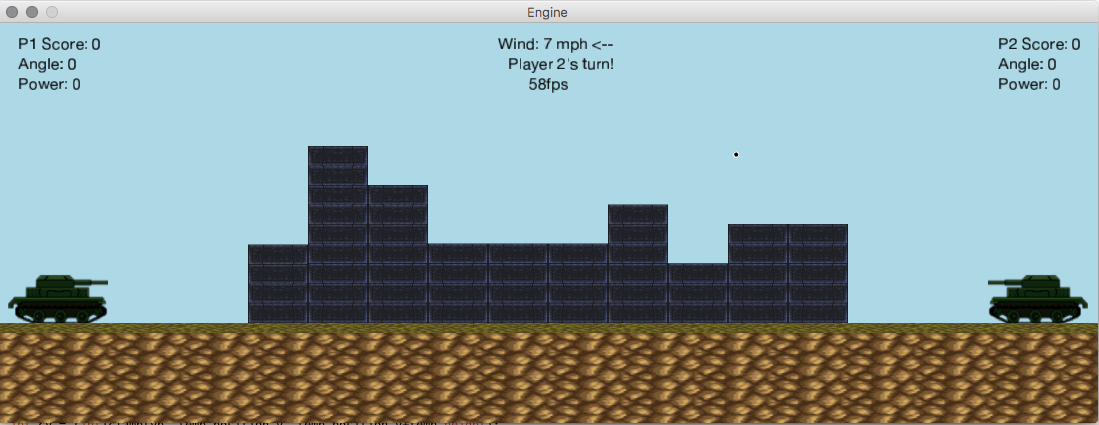
\includegraphics[width=17cm]{fired}}
\end{figure}

\section{Overview}
\subsection{Design}
At its bare-bones, the game is a simple particle system. All of the gameplay elements are particle objects. This made some of the physics calculations easy, but also has its limitations. For instance, the tank player characters are a subclass of Particle, but the texture that is layered on top of the particle is quite a complex polygon - so would be more suited to a less simplified representation of the object.
\par
The game features 2 players (as required) and each player has the ability to move forward and backward within their playing field. They also can draw a vector on screen from their tank to release a tank shell and fire it in the direction of the vector drawn. The tank shell is also a simple particle, with a radius (it is a circle) which eases collision calculations.
\par 
The terrain for the game is procedurally drawn at the start of each game, so it is different for each game. Also, the blocks are affected by the force of gravity, to add a sense of realism, so when a block is destroyed, the ones above it collapse in to fill the space.
\par 
To add a touch of flavour to the game, it was styled in a psuedo-World War 2 style, with textures and fonts that give a war aesthetic to the game. For this a start, end game, and hit detect screen were made. The introductory screen informs the users of the controls, the hit screen tells the users when a tank has been hit and which player scored, and the end game screen notifies that the game has ended and the winning player.
\subsection{Implementation}
The game is implemented using a class called \textbf{Game} which stores the current state of the game. As processing uses the draw() method at the start of each frame, this method calls game.tick() and game.render() respectively.
\par
\textbf{Game.tick()} is responsible for updating the forces on all active particles, then calling the integrate method on them, and finally collisions are detected. 
\par 
\textbf{Game.render()} is responsible for deciding what to draw to screen. Depending on what happened in the tick() call, boolean variables become set which allow the game to decide which screens to draw. All of the physics calculations are done in the tick phase, and render is only responsible for the graphics drawing.
\par 
The reason for the separation of the game into the 2 methods is that the graphics code and the physics should be completely separate, with the graphics only rendering the particles based on their positions which have been updated by the physics code. Thus, it is fairly easy to change the behaviour of code by altering the physics without affecting the graphics, and vice-versa.
\par 
The game elements are all subclasses of the \textbf{Particle} class, with each one adding/changing the implementation slightly to suit the needs of the particular game element that it is representing. This makes the collision detection code easier, as everything is just a single particle, as opposed to objects made out of aggregated particles. Forces on these particles are implemented using the force generator methodology, so each individual force has a class, with some of them taking constant values throughout the game, and some taking variable values depending on the state of the game (wind, tank acceleration).
\section{Play Area}
The play area is made up of 2 simple elements:
\begin{itemize}
\item Ground element
\item Grid of blocks
\end{itemize}
\begin{figure}[H]
\centerline{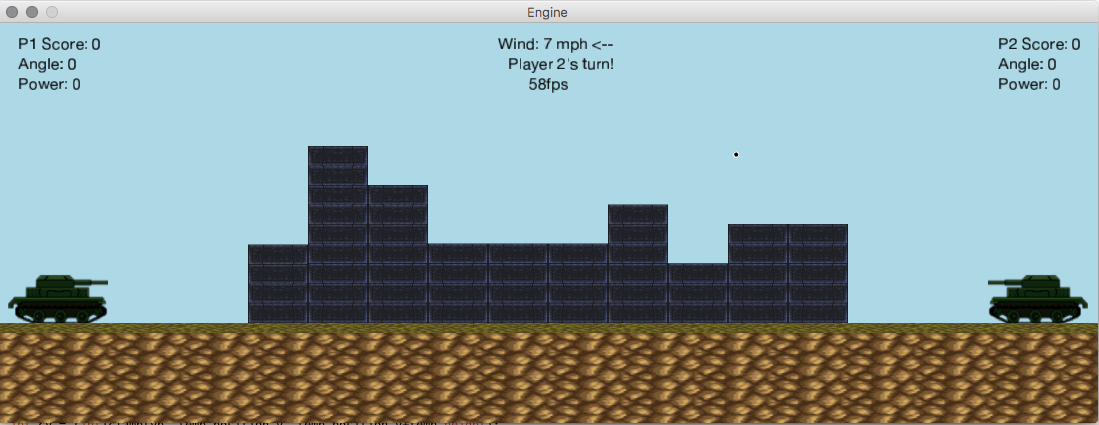
\includegraphics[width=17cm]{fired}}
\end{figure}
As can be seen in the image, the game's ground level is slightly up from the bottom of the game's floor. There is no particular reason for this other than the area is then free to add in textures. However, because the ground level is now not just at $ y = MAX\_HEIGHT $, there is some extra calculation involved in working out when a particle (or block) collides with the ground.
\par 
The ground is stored as an instance of the Plane object. Although a plane is a 3D object, the class is a simplified version of what would be used in a 3D game. Essentially the ground is a line, so to calculate when a projectile is coming into contact with the ground the vector of the incoming particle must be projected onto the ground's normal (the vector projecting at 90 degrees from the ground).
$$ dist = ClosingVector . GroundNormal $$
So if $ dist \leq projectile.radius $ then there is a collision with the ground.
\par 
The obstacles are implemented as a 2D array of the Block class. Block is a subclass of Particle, which also accepts a width and height as arguments for the constructor. Blocks of terrain are implemented as particles because the rectangular shape that represents the block can easily be stored as a particle in the top left corner, with the width and height describing the size of the box. This still allows for easy collision detection, the size of the box extending from the particle just needs to be taken into consideration.
\par 
\subsection{Design Decisions}
One of the major design decisions for the playing area was how to generate the terrain. The 2 options being to have either a fully static playing area that was the same at each new game, or to dynamically generate the terrain at the start of each new game. \par
\begin{minipage}[t]{0.5\textwidth}
\textbf{Advantages of Static}
\begin{itemize}
\item Easy to implement
\item Quick to generate
\end{itemize}
\textbf{Disadvantages of Static}
\begin{itemize}
\item Incredibly boring
\end{itemize}
\end{minipage}
\begin{minipage}[t]{0.5\textwidth}
\textbf{Advantages of Dynamic}
\begin{itemize}
\item Much more enjoyable
\item More of a challenge
\end{itemize}
\textbf{Disadvantages of Dynamic}
\begin{itemize}
\item Slower to generate
\end{itemize}
\end{minipage}
\par 
Clearly the easier option is to go with a static game field, but this is boring. From the outset it was decided that a dynamic field would be used. There are a fixed number of columns of blocks (which can be changed in code), but at game start up, these columns are filled with a dynamically generated array of blocks of a random length. It might have been even more pleasing to the player if something like the \textbf{noise} function had been used for the array length generation, as this would have produced a more well distributed set of array lengths, creating a more wave like pattern. However, it kind of fits in with the industrial look of the game to have random lengths for the arrays, as the block columns generated resemble buildings.
\par 
The block columns take up a set width of the game field, leaving 250 pixels on either side for the tanks. The columns are also limited in height, so that there is usable space for the players to fire projectiles into. The blocks use textures sourced for free online \cite{playTextures}
\par 
\textbf{Gravity \& Wind} were also major factors for the play area. Obviously gravity is constant anywhere in the game, so the gravity object is initialised in game setup with a vector value and left that way for the entire game. The value of the gravity is not the same as on earth (9.81ms$^{-1}$) but is instead a tuned value for the game. 
\par 
The wind force however is a constantly changing value. A timer is used to decide when to flip the wind value, then a random value within a certain range is selected and applied to the wind force generator. Likewise to gravity, the value of the wind force was also tuned for the game, but the UI prints out a user friendly value for the wind, as well as indicating which direction the wind is blowing in.
\section{Tanks}
As per the specification, there are 2 tanks - one for each player. Tanks (as mentioned before) are just particles, but have an associated width and height (like Blocks). As well as this, the tanks also have a \textbf{Max Speed} constant stored inside them. The reason for this being that tank movement is applied as an acceleration (as in real life) and the speed of the tanks then needs to be limited, or else they would continue to accelerate up the unbelievable speed. The tanks are rendered on screen using a texture found online for free \cite{tankTextures}.
\subsection{Design Decisions}
The tanks could have a number of choices for movement control e.g. mouse, keyboard. The decision was taken to use the keyboard, as the projectile is controlled using the mouse. It could easily have been done the other way round, however it is more common in games to use either WASD or the arrow keys to control vehicles, so in keeping with the spirit of gaming, the arrow keys are used to control the movement of tanks. As mentioned before, tank acceleration is done using a force generator, and the speed is capped.
\par 
Aiming of the tank is done with the mouse however, as the user draws a vector from the tank (see image). The angle and magnitude of this vector are displayed to the user in a human friendly format.
\begin{figure}[H]
\centerline{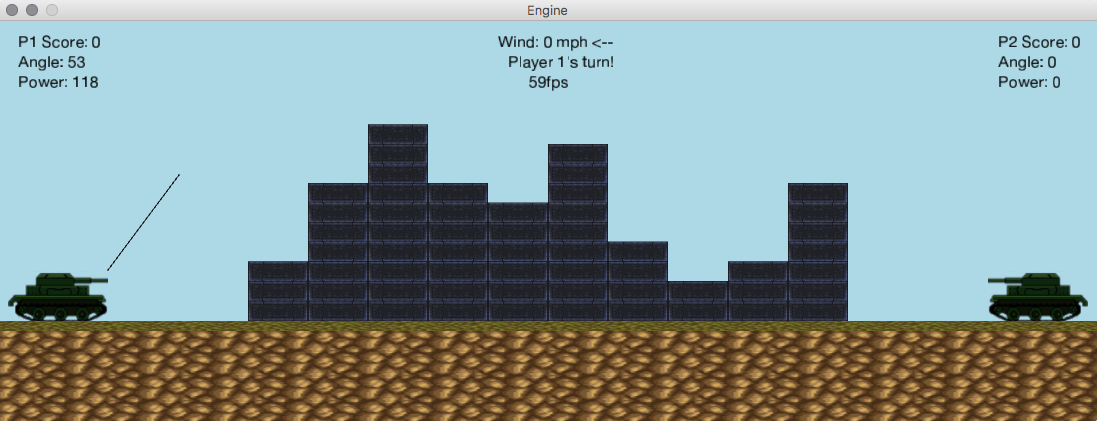
\includegraphics[width=17cm]{vector}}
\end{figure}
\par
As the tanks are just particles and are essentially just represented by rectangles with a texture laid on top, collision detection is fairly easy (and very similar to block collision detection).
\section{Projectile}
In the game, projectiles (as with everything else) are particles, however projectiles are circular particles, so have an associated radius. There is only ever one projectile in the game at a time, so it is stored in a varible in the game class for easy access in methods.
\subsection{Design Decisions}
The 2 main decisions for the game as far as projectiles are concerned are: the look of the shell, and the collision detection. To make the shell not look completely ridiculous, it should be kept in a size proportionate to the tanks. So for the selected size of the tanks, a shell of radius 5px was selected. This also makes collision detection quite simple, as it is easy to implement detection of a circular shell with the various flat edges of the game (blocks, ground, tanks).
\section{User Interface}
To make the game as user friendly as possible, it was necessary to do 2 things: add in all of the relevant information that a user would need, and texture the game so that it isn't completely boring to play.
\subsection{UI Elements}
There are a set of elements that needed to be included in the game to make it accessible to users. These include the current score of each player, the direction and size of the players fire vector, the player whose turn it currently is, and the wind.
\par 
On each side of the screen, each user is presented with their own score. Below this the users are told the angle and magnitude of their currently selected fire vector. As the players must draw the vector to fire the projectile, the values of the angle and power (magnitude) are 0 until it is the user's turn and they can then draw an appropriate vector onto the screen. 
\par 
The other information that the players need is displayed in the center of the screen, so that both players can see it clearly. This area shows the players whose turn it is, the current frame rate of the game (should they care) and also the strength and direction of the wind. As with the power and angle of the firing vector, the wind is displayed in a human friendly format (mph) and an arrow indicating the direction of the wind.
\begin{figure}[H]
\centerline{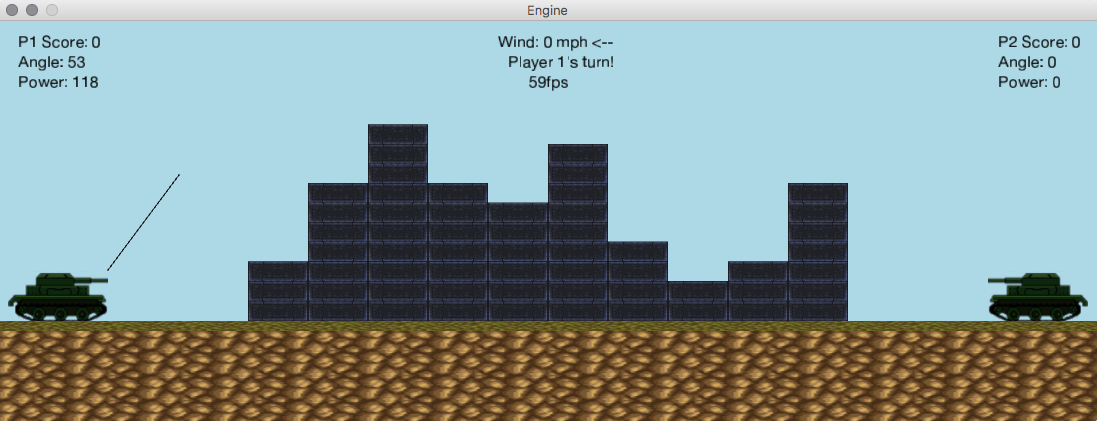
\includegraphics[width=17cm]{vector}}
\end{figure}
This image shows all of the UI elements. The angle and power are made into human friendly forms, as is the wind. Wind and power (magnitude) have maximum values and so the maximum speed for wind is 10mph and maximum shell power is 150 (although these are represented internally in completely different values).
\subsection{Game Screens}
The game has an introduction screen which tells the users how to control the game. It also offers some aesthetic value to the game. The title screen can be seen below:

\begin{figure}[H]
\centerline{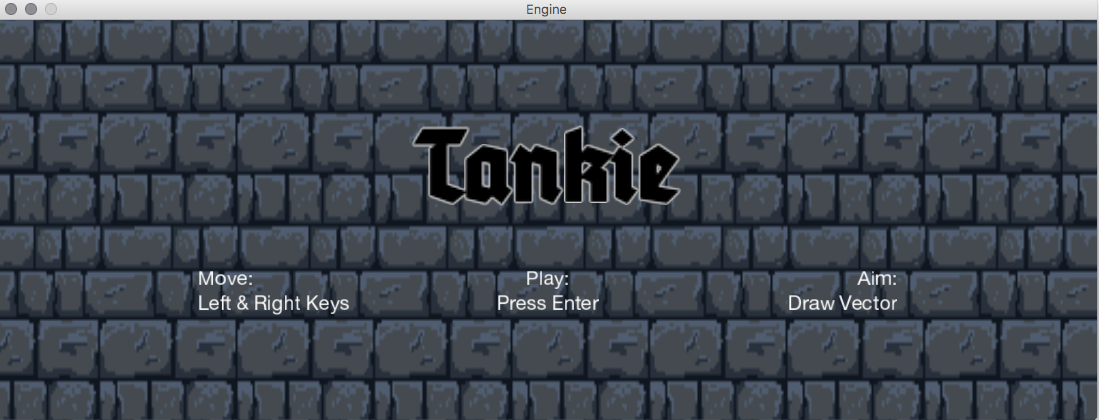
\includegraphics[width=17cm]{main}}
\end{figure}

As well as this, there are screens for a hit (seen below) which informs the users when a shell has collided with a tank, and also says which player scored. As well as this, there is also a game over screen.

\begin{figure}[H]
\centerline{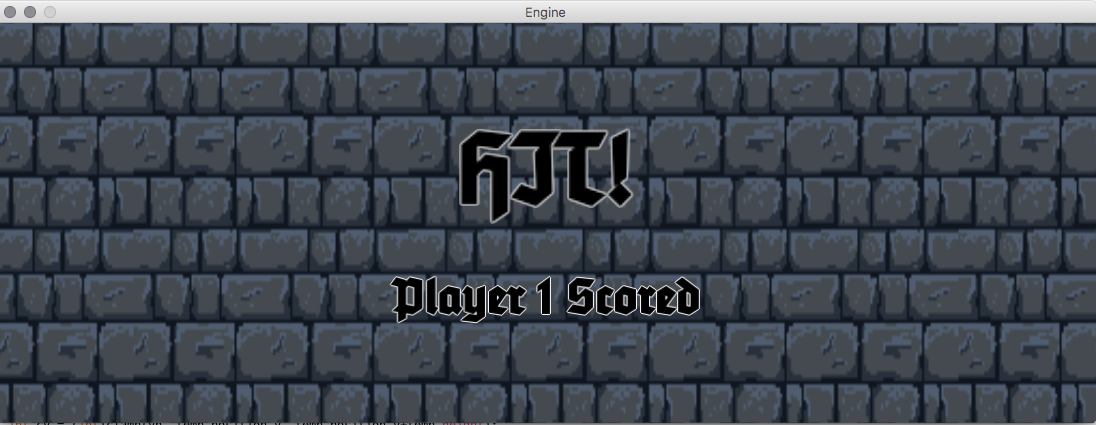
\includegraphics[width=17cm]{hit}}
\end{figure}

\section{Physics}
The physics system in the game is based on particles and force generators. The basics of the particle class and force generators were taken from the code given in class \cite{code}. The particle class is used as the basis for all objects in the game. Particular mention must be drawn to the tank class. It contains a constant which represents the maximum speed of the tanks, as it should not be able to accelerate forever. This is used in the \textbf{tank.integrate()} method as such
\begin{lstlisting}
// Clip speed to within the max speed range.
if(velocity.mag() > MAX_SPEED){
 velocity.normalize();
 velocity.mult(MAX_SPEED);
}
\end{lstlisting}
\par
Particles are affected by forces, and each particle can be acted upon by multiple forces at once. Each force is represented by a force generator of the appropriate type. These are then registered to a particle using the \textbf{ForceRegistry} class. Unlike the code given, the implementation of \textbf{ForceRegistry} used in the game instead uses a \textbf{HashMap} to store the registrations - the key of the registry is the force, and the value is an arraylist of particles on which to apply the force. This means that search time to find a particular force in the registry is much lower, assuming we need to remove a particle from a force.
\par 
The forces in the game are:
\begin{itemize}
\item Gravity - tuned to game
\item Wind - set randomly at intervals
\item Tank Acceleration - turned on and off with key presses
\end{itemize}
Gravity acts on all particles in the game apart from tanks (this is because the tanks cannot change elevation, so only moving on flat ground requires no gravity). Wind only acts on the projectiles because both the blocks of scenery and the tanks are much to heavy for wind to have an effect. As for the tank acceleration, that only acts on tanks, and it is only applied when the user is holding down the arrow keys for that direction of movements.
\par 
\subsection{Collisions}
The collision contact code is taken from the class provided code \cite{code} and also from the book \cite{book}. As per the book's suggestions, collisions of non-moving objects with the ground are treated as resting contacts - thus, all blocks at the bottom of the columns are in resting contact with the ground (which is represented as a line across the screen). 
\par 
To detect collision (or resting contact) with the ground level, it was decided that just hard-coding in the height of the ground to the particle class like so:
\begin{lstlisting}
if((position.y > GROUND_LEVEL)) velocity.y = -velocity.y
\end{lstlisting}
is a terrible idea, as it is not a good physics representation of the ground. Instead the \textbf{Plane} class was created which represents the 2D plane of the ground in the game. Collisions with the ground are then found by examining the projection of a vector closing in on the ground level onto the ground's normal vector (as mentioned above). 
$$ Dist = projection $$
$$ projection = |ClosingVector| cos \theta  $$
$$ |ClosingVector| cos \theta = ClosingVector \cdot Normal $$
So if the distance (magnitude) of a vector closing in on the ground was less than the size of the object it represented, a contact was generated. Collisions with the ground of any particles are done using this method.
\par 
For collision with blocks and tanks, a similar method is used. The \textbf{Clamp} method in the Game class is used to determine which part of an object is closest to the incoming particle (since all objects in the game are rectangles (bar the projectile)). A vector is then found between the closest part of the object and then incoming particle, and if the magnitude of this vector is less than or equal to the particle's width then a collision is generated.
\section{Extensions}
\subsection{Gravity on Blocks}
Gravity on blocks was implemented as an extension. To do this, blocks must have a mass, because if they had no or infinite mass, then gravity would not affect them in game. As such, blocks are given a mass for the gravity calculations, but when tanks collide with blocks, they are treated as infinite mass and do not experience an impulse as a result of the collision.
\begin{figure}[H]
\centerline{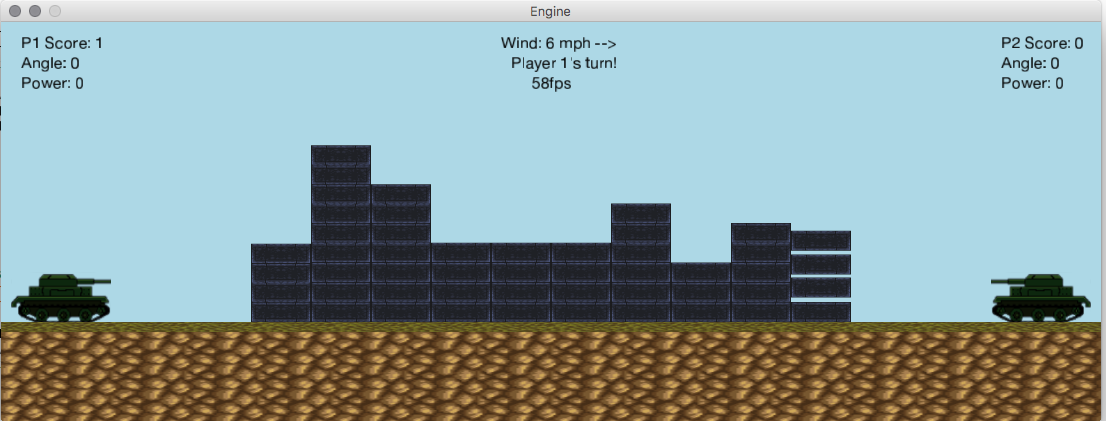
\includegraphics[width=17cm]{gravity}}
\end{figure}
As can be seen in the image, when a block is destroyed, it is removed from the game, and the blocks above it are pulled down by the force of gravity that they experience. However, the blocks are all separate, and not stuck together, so when a column of blocks falls, they appear to separate and then come together again.
\par 
When blocks collide with each other after falling down, they undergo completely inelastic collision. This is not completely true to life, as there would be a little spring in the collisions between large blocks and the ground. However, the springing effect would be quite slight, so it is an imaginable simplification to just have inelastic collisions and make the particles experience no impulse other than the impulse required to stop them from going through each other or the ground.
\subsection{Tank Acceleration}
As a slight extension to tank movement, instead of treating tank movement as just an update to the tank's position vector, the movement is done through force generators. When the user presses the key to move a tank, the force generator for that tank is given a value. This in turn gives the tank an acceleration. However, to prevent the tank from accelerating indefinitely, the tank is also given a maximum speed (as mentioned before). During the integrate step, if the maximum speed is reached, then the velocity vector of the tank is normalised and multiplied by the maximum speed to make sure that the maximum is never exceeded.
\subsection{Textures and Screens}
To add some spice to the game, various textures have been used. As well as this, some screens have been made to give information to the users. However, collision detection with the tanks is a little bit off, because the tank textures contain blank space, but the tanks are represented as rectangles in the game (for ease). So to implement collision detection on tanks properly, they should either be stored as polygons made up of particles, or the engine should be re-written entirely so that it is not a mass-aggregate engine.
\subsection{Sounds}
Some simple sound affects for firing the shell, and the shell exploding, were also implemented using the minim library.


\begin{thebibliography}{9}
\bibitem{playTextures}
  \textbf{http://opengameart.org/content/lots-of-free-2d-tiles-and-sprites-by-hyptosis}
  \emph{2D textures used for play area},
  accessed 22/09/16

\bibitem{tankTextures}
  \textbf{http://opengameart.org/content/2d-side-scrolling-tank}
  \\
  \emph{Tank textures},
  accessed on 22/09/16
  
\bibitem{code}
   \textbf{Processing Particle Physics Code}\\
   \emph{Ian Miguel \& Chris Jefferson}
   Studres
\bibitem{book}
   \textbf{Game Engine Physics Development}\\
   \emph{Ian Millington},
   Morgan Kaufman Publishing, 2007
\end{thebibliography}
\end{document}
